\documentclass[tikz]{standalone}

\begin{document}
  \tikzset{>=latex} % Change default arrowhead to filled triangle
  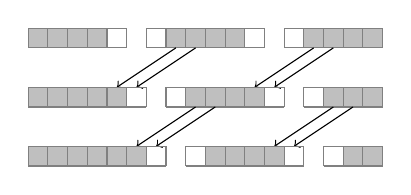
\begin{tikzpicture}[scale=0.25]

    
    % transarray[vOffset, hShift]
    \def\transarray[#1, #2]{
    \fill[lightgray] (0,#1) rectangle (#2+4,#1+1);
    \draw[gray, step=1] (0,#1) grid (#2+5,#1+1);
    
    \fill[lightgray] (#2+7,#1) rectangle (#2+11,#1+1);
    \draw[gray, step=1] (#2+6,#1) grid (#2+12,#1+1);
    
    \fill[lightgray] (#2+14,#1) rectangle (18,#1+1);
    \draw[gray, step=1] (#2+13,#1) grid (18,#1+1);
    }


    % transarrows[vOffset, hShift]
    \def\transarrows[#1, #2]{
      % Arrows
      \draw[->](#2+4.5,#1+2) to (#2+1.5,#1);
      \draw[->](#2+3.5,#1+2) to (#2+0.5,#1);

      \draw[->](#2+11.5,#1+2) to (#2+8.5,#1);
      \draw[->](#2+10.5,#1+2) to (#2+7.5,#1);
    }
    
    \transarray[6, 0]
    \transarrows[4, 4]
    \transarray[3, 1]
    \transarrows[1, 5]
    \transarray[0, 2]

  \end{tikzpicture}
\end{document}
